\begin{figure}
    \begin{adjustbox}{width=\textwidth}
    \tikzset{every picture/.style={line width=0.75pt}} %set default line width to 0.75pt        
    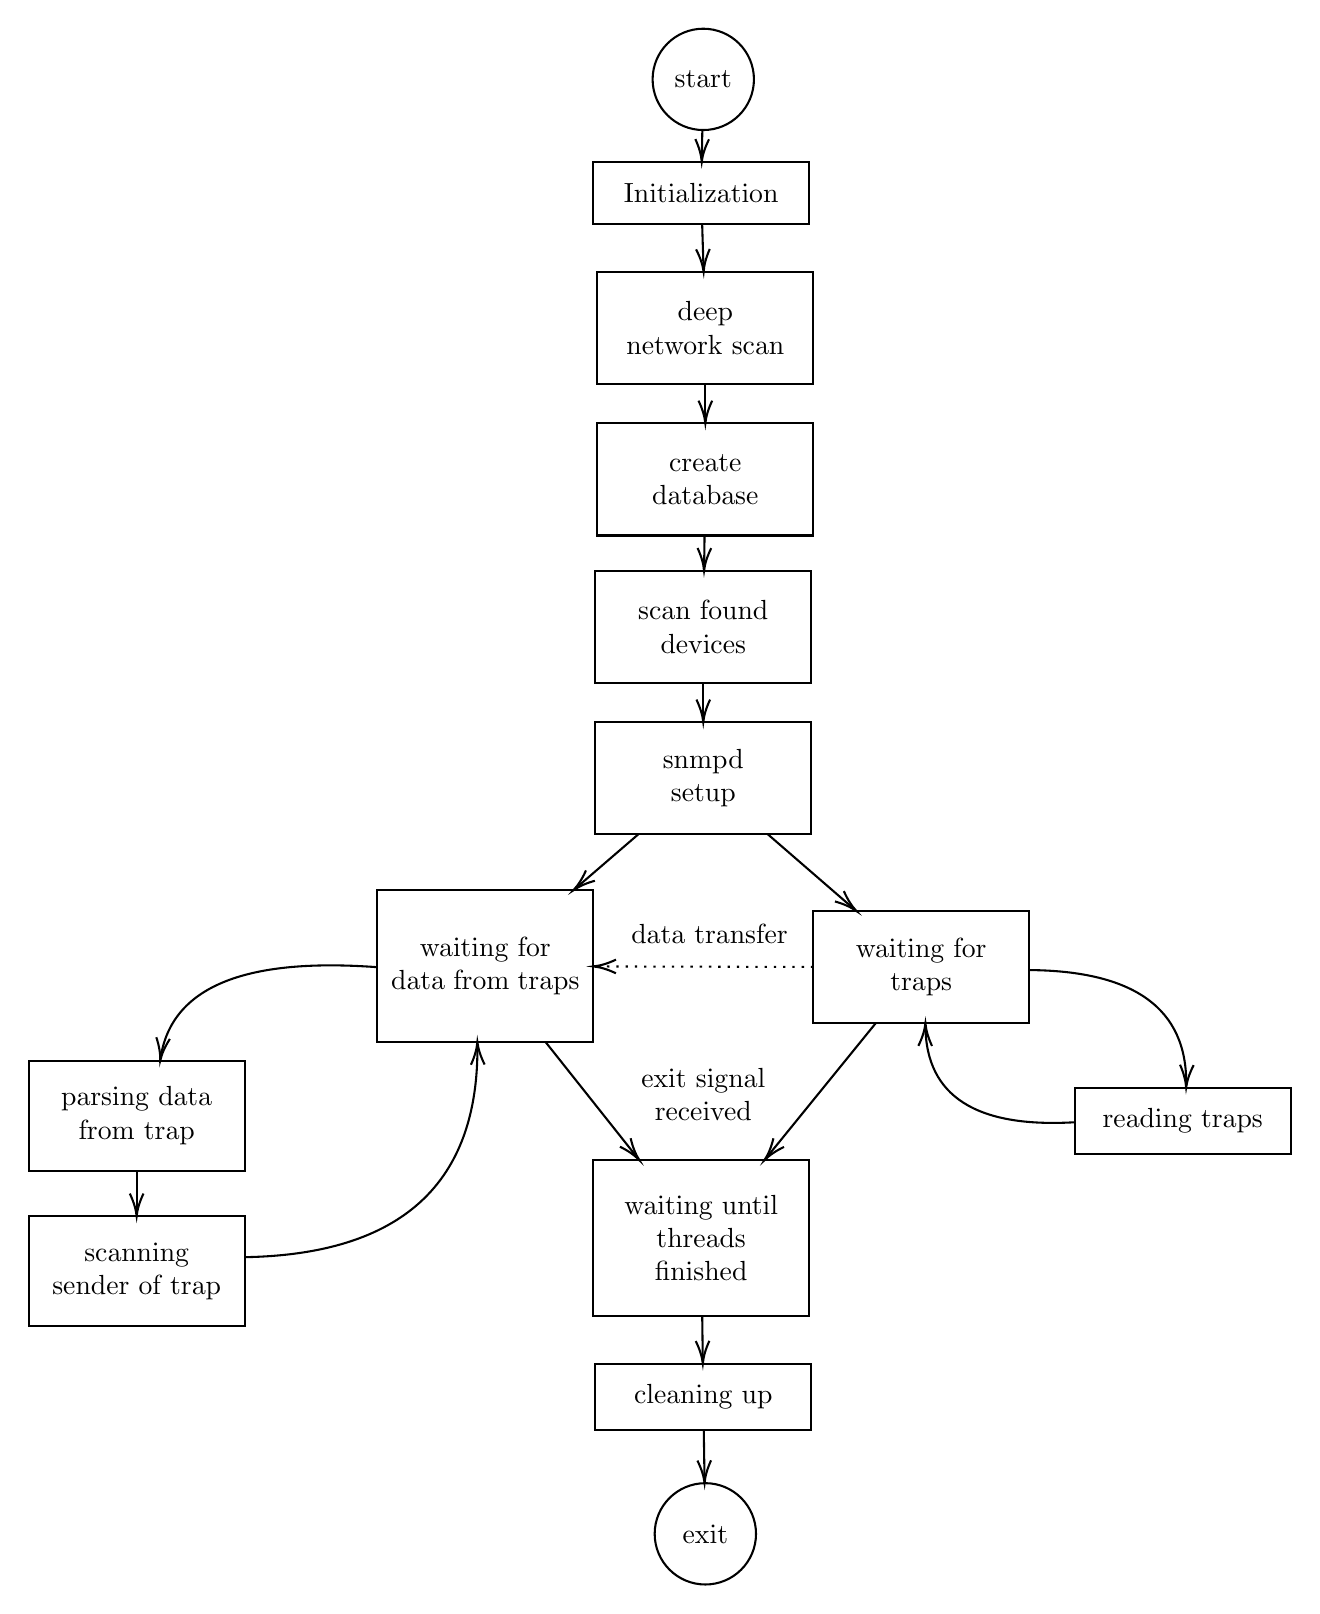
\begin{tikzpicture}[x=0.75pt,y=0.75pt,yscale=-1,xscale=1]
        %uncomment if require: \path (0,768); %set diagram left start at 0, and has height of 768
        
        % Text Node
        \draw    (304,65.75) -- (408,65.75) -- (408,95.75) -- (304,95.75) -- cycle  ;
        \draw (356,80.75) node   [align=left] {\begin{minipage}[lt]{68pt}\setlength\topsep{0pt}
        \begin{center}
        Initialization
        \end{center}
        
        \end{minipage}};
        % Text Node
        \draw    (306,118.75) -- (410,118.75) -- (410,172.75) -- (306,172.75) -- cycle  ;
        \draw (358,145.75) node   [align=left] {\begin{minipage}[lt]{68pt}\setlength\topsep{0pt}
        \begin{center}
        deep\\network scan
        \end{center}
        
        \end{minipage}};
        % Text Node
        \draw    (306,191.75) -- (410,191.75) -- (410,245.75) -- (306,245.75) -- cycle  ;
        \draw (358,218.75) node   [align=left] {\begin{minipage}[lt]{68pt}\setlength\topsep{0pt}
        \begin{center}
        create\\database
        \end{center}
        
        \end{minipage}};
        % Text Node
        \draw    (305,262.75) -- (409,262.75) -- (409,316.75) -- (305,316.75) -- cycle  ;
        \draw (357,289.75) node   [align=left] {\begin{minipage}[lt]{68pt}\setlength\topsep{0pt}
        \begin{center}
        scan found devices
        \end{center}
        
        \end{minipage}};
        % Text Node
        \draw    (305,335.75) -- (409,335.75) -- (409,389.75) -- (305,389.75) -- cycle  ;
        \draw (357,362.75) node   [align=left] {\begin{minipage}[lt]{68pt}\setlength\topsep{0pt}
        \begin{center}
        snmpd\\setup
        \end{center}
        
        \end{minipage}};
        % Text Node
        \draw    (410,426.75) -- (514,426.75) -- (514,480.75) -- (410,480.75) -- cycle  ;
        \draw (462,453.75) node   [align=left] {\begin{minipage}[lt]{68pt}\setlength\topsep{0pt}
        \begin{center}
        waiting for\\traps
        \end{center}
        
        \end{minipage}};
        % Text Node
        \draw    (200,416.75) -- (304,416.75) -- (304,489.75) -- (200,489.75) -- cycle  ;
        \draw (252,453.25) node   [align=left] {\begin{minipage}[lt]{68pt}\setlength\topsep{0pt}
        \begin{center}
        waiting for\\data from traps
        \end{center}
        
        \end{minipage}};
        % Text Node
        \draw    (32,498.75) -- (136,498.75) -- (136,551.75) -- (32,551.75) -- cycle  ;
        \draw (84,525.25) node   [align=left] {\begin{minipage}[lt]{68pt}\setlength\topsep{0pt}
        \begin{center}
        parsing data from trap
        \end{center}
        
        \end{minipage}};
        % Text Node
        \draw    (32,573.75) -- (136,573.75) -- (136,626.75) -- (32,626.75) -- cycle  ;
        \draw (84,600.25) node   [align=left] {\begin{minipage}[lt]{68pt}\setlength\topsep{0pt}
        \begin{center}
        scanning sender of trap
        \end{center}
        
        \end{minipage}};
        % Text Node
        \draw    (536,511.75) -- (640,511.75) -- (640,543.75) -- (536,543.75) -- cycle  ;
        \draw (588,527.75) node   [align=left] {\begin{minipage}[lt]{68pt}\setlength\topsep{0pt}
        \begin{center}
        reading traps
        \end{center}
        
        \end{minipage}};
        % Text Node
        \draw    (304,546.75) -- (408,546.75) -- (408,621.75) -- (304,621.75) -- cycle  ;
        \draw (356,584.25) node   [align=left] {\begin{minipage}[lt]{68pt}\setlength\topsep{0pt}
        \begin{center}
        waiting until threads finished
        \end{center}
        
        \end{minipage}};
        % Text Node
        \draw    (305,644.75) -- (409,644.75) -- (409,676.75) -- (305,676.75) -- cycle  ;
        \draw (357,660.75) node   [align=left] {\begin{minipage}[lt]{68pt}\setlength\topsep{0pt}
        \begin{center}
        cleaning up
        \end{center}
        
        \end{minipage}};
        % Text Node
        \draw    (358, 726.75) circle [x radius= 24.41, y radius= 24.41]   ;
        \draw (358,726.75) node   [align=left] {\begin{minipage}[lt]{25.84pt}\setlength\topsep{0pt}
        \begin{center}
        exit
        \end{center}
        
        \end{minipage}};
        % Text Node
        \draw    (357, 26) circle [x radius= 24.41, y radius= 24.41]   ;
        \draw (357,26) node   [align=left] {\begin{minipage}[lt]{25.84pt}\setlength\topsep{0pt}
        \begin{center}
        start
        \end{center}
        
        \end{minipage}};
        % Text Node
        \draw (357,515) node   [align=left] {\begin{minipage}[lt]{68pt}\setlength\topsep{0pt}
        \begin{center}
        exit signal\\received
        \end{center}
        
        \end{minipage}};
        % Text Node
        \draw (360,437.75) node   [align=left] {\begin{minipage}[lt]{68pt}\setlength\topsep{0pt}
        \begin{center}
        data transfer
        \end{center}
        
        \end{minipage}};
        % Connection
        \draw    (356.46,95.75) -- (357.11,116.75) ;
        \draw [shift={(357.17,118.75)}, rotate = 268.24] [color={rgb, 255:red, 0; green, 0; blue, 0 }  ][line width=0.75]    (10.93,-3.29) .. controls (6.95,-1.4) and (3.31,-0.3) .. (0,0) .. controls (3.31,0.3) and (6.95,1.4) .. (10.93,3.29)   ;
        % Connection
        \draw    (358,172.75) -- (358,189.75) ;
        \draw [shift={(358,191.75)}, rotate = 270] [color={rgb, 255:red, 0; green, 0; blue, 0 }  ][line width=0.75]    (10.93,-3.29) .. controls (6.95,-1.4) and (3.31,-0.3) .. (0,0) .. controls (3.31,0.3) and (6.95,1.4) .. (10.93,3.29)   ;
        % Connection
        \draw    (357.62,245.75) -- (357.41,260.75) ;
        \draw [shift={(357.38,262.75)}, rotate = 270.81] [color={rgb, 255:red, 0; green, 0; blue, 0 }  ][line width=0.75]    (10.93,-3.29) .. controls (6.95,-1.4) and (3.31,-0.3) .. (0,0) .. controls (3.31,0.3) and (6.95,1.4) .. (10.93,3.29)   ;
        % Connection
        \draw    (357,316.75) -- (357,333.75) ;
        \draw [shift={(357,335.75)}, rotate = 270] [color={rgb, 255:red, 0; green, 0; blue, 0 }  ][line width=0.75]    (10.93,-3.29) .. controls (6.95,-1.4) and (3.31,-0.3) .. (0,0) .. controls (3.31,0.3) and (6.95,1.4) .. (10.93,3.29)   ;
        % Connection
        \draw    (388.15,389.75) -- (429.33,425.44) ;
        \draw [shift={(430.85,426.75)}, rotate = 220.91] [color={rgb, 255:red, 0; green, 0; blue, 0 }  ][line width=0.75]    (10.93,-3.29) .. controls (6.95,-1.4) and (3.31,-0.3) .. (0,0) .. controls (3.31,0.3) and (6.95,1.4) .. (10.93,3.29)   ;
        % Connection
        \draw    (325.67,389.75) -- (295.86,415.44) ;
        \draw [shift={(294.35,416.75)}, rotate = 319.24] [color={rgb, 255:red, 0; green, 0; blue, 0 }  ][line width=0.75]    (10.93,-3.29) .. controls (6.95,-1.4) and (3.31,-0.3) .. (0,0) .. controls (3.31,0.3) and (6.95,1.4) .. (10.93,3.29)   ;
        % Connection
        \draw    (440.07,480.75) -- (387.72,545.2) ;
        \draw [shift={(386.46,546.75)}, rotate = 309.09] [color={rgb, 255:red, 0; green, 0; blue, 0 }  ][line width=0.75]    (10.93,-3.29) .. controls (6.95,-1.4) and (3.31,-0.3) .. (0,0) .. controls (3.31,0.3) and (6.95,1.4) .. (10.93,3.29)   ;
        % Connection
        \draw    (280.98,489.75) -- (324.99,545.18) ;
        \draw [shift={(326.23,546.75)}, rotate = 231.55] [color={rgb, 255:red, 0; green, 0; blue, 0 }  ][line width=0.75]    (10.93,-3.29) .. controls (6.95,-1.4) and (3.31,-0.3) .. (0,0) .. controls (3.31,0.3) and (6.95,1.4) .. (10.93,3.29)   ;
        % Connection
        \draw    (356.49,621.75) -- (356.76,642.75) ;
        \draw [shift={(356.79,644.75)}, rotate = 269.25] [color={rgb, 255:red, 0; green, 0; blue, 0 }  ][line width=0.75]    (10.93,-3.29) .. controls (6.95,-1.4) and (3.31,-0.3) .. (0,0) .. controls (3.31,0.3) and (6.95,1.4) .. (10.93,3.29)   ;
        % Connection
        \draw    (357.24,676.75) -- (357.6,700.34) ;
        \draw [shift={(357.63,702.34)}, rotate = 269.13] [color={rgb, 255:red, 0; green, 0; blue, 0 }  ][line width=0.75]    (10.93,-3.29) .. controls (6.95,-1.4) and (3.31,-0.3) .. (0,0) .. controls (3.31,0.3) and (6.95,1.4) .. (10.93,3.29)   ;
        % Connection
        \draw    (200,453.75) .. controls (135.65,448.98) and (100.84,463.46) .. (95.59,497.2) ;
        \draw [shift={(95.37,498.75)}, rotate = 277.23] [color={rgb, 255:red, 0; green, 0; blue, 0 }  ][line width=0.75]    (10.93,-3.29) .. controls (6.95,-1.4) and (3.31,-0.3) .. (0,0) .. controls (3.31,0.3) and (6.95,1.4) .. (10.93,3.29)   ;
        % Connection
        \draw    (514,455.13) .. controls (564.8,455.49) and (590.02,473.81) .. (589.68,510.08) ;
        \draw [shift={(589.65,511.75)}, rotate = 271.74] [color={rgb, 255:red, 0; green, 0; blue, 0 }  ][line width=0.75]    (10.93,-3.29) .. controls (6.95,-1.4) and (3.31,-0.3) .. (0,0) .. controls (3.31,0.3) and (6.95,1.4) .. (10.93,3.29)   ;
        % Connection
        \draw    (536,528.45) .. controls (488.38,531.25) and (464.39,515.86) .. (464.04,482.3) ;
        \draw [shift={(464.04,480.75)}, rotate = 90.62] [color={rgb, 255:red, 0; green, 0; blue, 0 }  ][line width=0.75]    (10.93,-3.29) .. controls (6.95,-1.4) and (3.31,-0.3) .. (0,0) .. controls (3.31,0.3) and (6.95,1.4) .. (10.93,3.29)   ;
        % Connection
        \draw    (84,551.75) -- (84,571.75) ;
        \draw [shift={(84,573.75)}, rotate = 270] [color={rgb, 255:red, 0; green, 0; blue, 0 }  ][line width=0.75]    (10.93,-3.29) .. controls (6.95,-1.4) and (3.31,-0.3) .. (0,0) .. controls (3.31,0.3) and (6.95,1.4) .. (10.93,3.29)   ;
        % Connection
        \draw    (136,593.46) .. controls (211.62,592.16) and (249.02,557.92) .. (248.17,490.76) ;
        \draw [shift={(248.16,489.75)}, rotate = 88.96] [color={rgb, 255:red, 0; green, 0; blue, 0 }  ][line width=0.75]    (10.93,-3.29) .. controls (6.95,-1.4) and (3.31,-0.3) .. (0,0) .. controls (3.31,0.3) and (6.95,1.4) .. (10.93,3.29)   ;
        % Connection
        \draw    (356.55,50.41) -- (356.31,63.75) ;
        \draw [shift={(356.27,65.75)}, rotate = 271.05] [color={rgb, 255:red, 0; green, 0; blue, 0 }  ][line width=0.75]    (10.93,-3.29) .. controls (6.95,-1.4) and (3.31,-0.3) .. (0,0) .. controls (3.31,0.3) and (6.95,1.4) .. (10.93,3.29)   ;
        % Connection
        \draw  [dash pattern={on 0.84pt off 2.51pt}]  (410,453.63) -- (306,453.38) ;
        \draw [shift={(304,453.37)}, rotate = 0.14] [color={rgb, 255:red, 0; green, 0; blue, 0 }  ][line width=0.75]    (10.93,-3.29) .. controls (6.95,-1.4) and (3.31,-0.3) .. (0,0) .. controls (3.31,0.3) and (6.95,1.4) .. (10.93,3.29)   ;
    \end{tikzpicture}
    \end{adjustbox}
    \caption{Program flow of the application.}
    \label{Figure:Application-StateMachine}
\end{figure}